\documentclass{article}

\usepackage[ngerman]{babel}
\usepackage[utf8]{inputenc}
\usepackage[T1]{fontenc}
\usepackage{tikz}
\usetikzlibrary{positioning, arrows}
\usepackage{listings}
\usepackage{fancybox}
\usepackage{fancyhdr}
\usepackage{lastpage}
\usepackage{verbatim}
\usepackage{ulem}
\usepackage{float}
\usepackage{hyperref}

\title{Meilenstein}
\pagestyle{fancy}
\fancyhf{}

%\usepackage{geometry}
%\geometry{a4paper,left=40mm,right=30mm, top=2cm, bottom=4cm} 


\lhead{Seite:\thepage / \pageref{LastPage}}
\rhead{Gruppe: swp15.gkp}
\chead{1. Meilenstein}

\renewcommand{\headrulewidth}{0.4pt}
%\renewcommand{\footrulewidth}{0.4pt}

\author{swp15.gkp}
\date{\today{}}
%\logo{\includegraphics[scale=0.25]{logo}}
\begin{comment}
1)Komponenten unvollständig 
     API als Datenbankzugriffsschicht 
     Verbindung zu Realdaten genauer beschreiben 
     Speicherung von Spielkarten, Spieler und Highscores als URI im Triple Store 
2)Architekturdiagramm für Layer 
!3)formale Spielregeln mit Quellenangabe für Implementation der Logik 
4)zweites Regelwerk für Kartenerzeugung 
evtl. Einschränkung auf bestimmte Städte 
5)Interface genauer beschreiben, so dass Implementation abgeleitet werden kann 
6)minimale Software und Liste an Kann-Funktionalitäten 
      Spezifikation von Abnahmekriterien 


Abgabe: nach der Prüfungszeit 

\end{comment}



\begin{document}
{\center \huge \textbf{Kartenbasiertes Multiplayerspiel}} \\ 
\center \huge Pac-Man aka "Pucman"

\flushleft 
\normalsize
\tableofcontents

\section{Zu uns und unserer Arbeitsweise:}
\begin{itemize}
\item Scum als Vorgehensrahmen
\item verschiedene Rollen je nach individueller Erfahrung
\end{itemize}
\begin{figure}[htb]
  \centering
  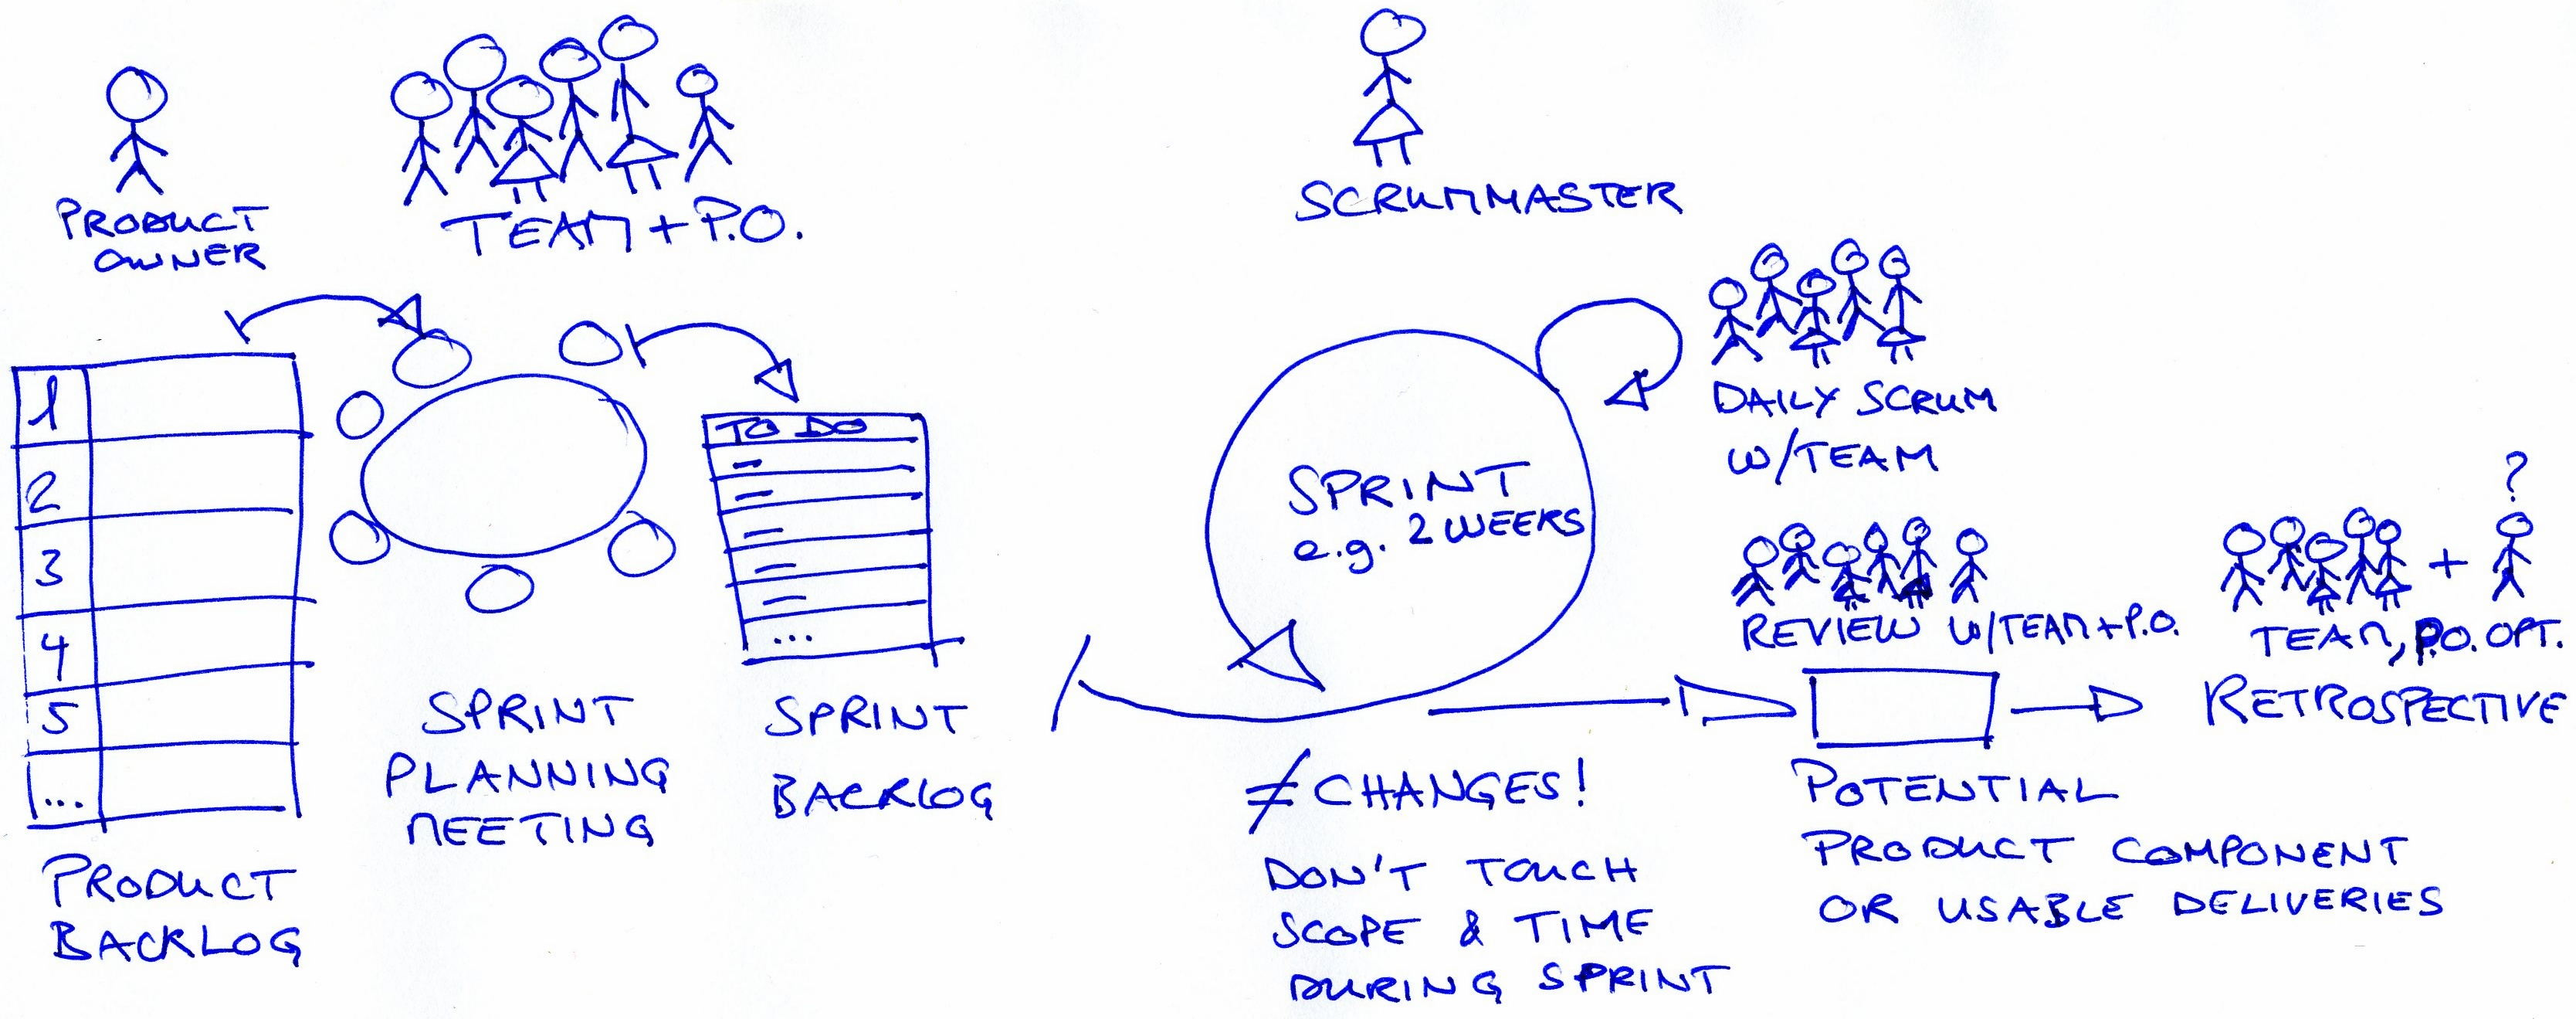
\includegraphics[scale=0.1]{Scrum.jpg}
%\caption{der rote Punkt bezeichnet unser gesuchtes Teilwort}
  \label{PNFs}
\end{figure} 
\flushleft 

%\end{frame}
\section{Projektvision}
\subsection{Was wollen wir erschaffen?}
\begin{itemize}
\item Pac-Man auf einen realen Kartenausschnitt
spielen
\item mit anderen Spielern zusammen spielen
\item Highscores mit denen anderer
vegleichen
\item das ganze als Browsergame
\end{itemize}

\subsection{Funktionalität der Webapplikation}
Das Programm wird als eine Web 3 Schichtenarchitektur umgesetzt.
\begin{enumerate}
\item Webclient
\item Webserver
\item Datenserver
\end{enumerate}

\subsection{Architekturdiagramm}
\begin{figure}[H]
  \centering
  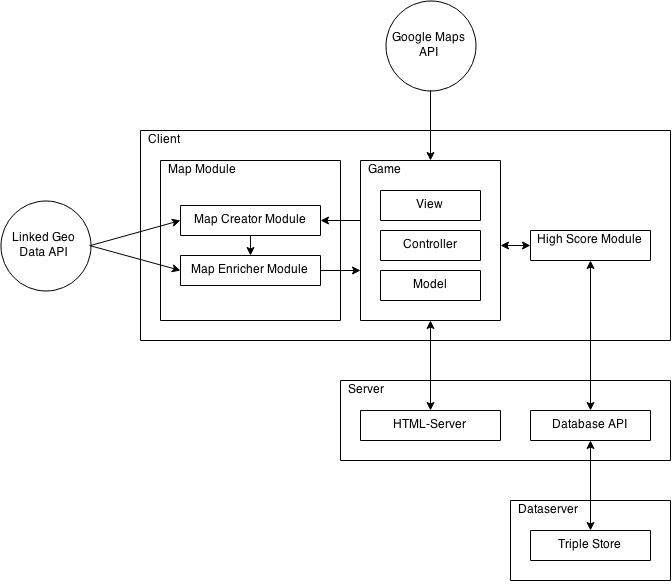
\includegraphics[scale=0.5]{arch.png}
%\caption{der rote Punkt bezeichnet unser gesuchtes Teilwort}
  \label{PNFs}
\end{figure} 


\section{Webclient}
Der Webclient ist der Browser des Anwenders, der die Website aufruft und die Javascript-Dateien die vom Webserver kommen ausführt. 

\subsection{Spielelogik}
Die Spielelogik ist im Quelltext implementiert.
Es folgt eine ausführliche Beschreibung als Vorlage für die Implementierung.
\subsubsection{Minimalanforderung}
Die Spielfigur (Pac-Man) muss Punkte in einem Labyrinth fressen, während
sie von Gespenstern verfolgt wird.\\
Der Weg den Pac-Man gehen kann, ist durch Mauern begrenzt. Alle Stellen,
an denen keine Mauer steht, kann von Pac-Man begangen werden. Dem
Spieler stehen zur Navigation die Cursortasten (Pfeil rechts, Pfeil
links, Pfeil oben, Pfeil unten) zur Verfügung. Mit diesen steuert er
Pac-Man analog zu den Pfeilrichtungen durch das Labyrinth.\\
In einem Teil des Labyrinths befindet sich ein durch Mauern
eingegrenztes Rechteck mit nur einem schmalen Durchgang. Wir bezeichnen
diesen Bereich als Gefängnis.\\
Es existieren im Spiel 4 Gespenster. Bei Levelbeginn befinden sich diese
im Gefängnis. Diese haben unterschiedliche Namen, unterschiedliche
Farben, und bewegen sich nach jeweils unterschiedlichen, vorgegebenen
Mustern.\\
- Oikabe (Verfolger, Farbe Rot)\\
Oikabe bewegt sich zunächst bedingt zufallsgesteuert. Erreicht er eine
Wand, auf die er zuläuft, entscheidet er sich zufällig in welche
Richtung er weiterläuft. Läuft er an einer Abzweigung vorbei, läuft er
geradeaus weiter. Sobald Pac-Man sich in einer geraden Linie vor Oikabe
in der Laufrichtung von Oikabe, befindet, und es ist kein unbegehbares
Hidnernis mehr zwischen Pac-Man und Oikabe, bezeichnen wir diesen
Vorgang wie folgt: Oikabe sieht Pac-Man. Solange Oikabe Pac-Man sieht,
verfolgt er Pac-Man. er läuft ihm solange hinterher wie er ihn sehen
kann beziwehungsweise bis er Pac-Man gefressen hat. \\
- Machibuse (Hinterhalt, Pink)\\
Machibuse's Bewegung zielt darauf ab, sich vor Pac-Man in den Weg zu
stellen. Er versucht sich immer in Laufrichtung von Pac-Man vor Ihm zu
positionieren.\\
- Otoboke (Dummkopf, Orange)\\
Otoboke ist der einzige Geist, der sich durchweg zufällig bewegt. Er
entscheidet sich an jeder Entscheidungsmöglichkeit zufällig, welche
Richtung er als nächstes einschlägt.\\
- Kimagure (launisch, Hellblau)\\
Die Bewegung von Kimagure ist eine zufällige Mischung aus zufälliger
Bewegung und dem Bewegungsmuster von Machibuse, er ist als eine Mischung
aus Otoboke und Machibuse.\\
Sobald sich die Position von Pac-Man und einem (oder auch mehreren
Geistern) überschneiden, verliert der Spieler ein Leben und Pac-Man
wird, nach einem kurzen Countdown, an seiner Ausgangsposition wieder
eingesetzt (gespawnt). Diesen Vorgang bezeichnen wir als: Pac-Man wird
gefressen. \\
Bei Levelbeginn besteht der gesamte begehbare Bereich, ausgenommen das
Gefängnis, aus Punkten die zum Bestehen des Levels von Pac-Man gefressen
werden müssen. Als Fressen bezeichnen wir den Vorgang, dass Pac-Man über
einen Punkt hinwegbewegt wird. ist Pac-Man zu mehr als 50\% über einem
Punkt hinweg gelaufen, wird dem Spieler eine Punkt zugerechnet und der
Punkt verschwindet.\\
\subsubsection{Optionale Eigenschaften}
Ein Teil der Punkte (ca. 4 Pro Level) haben einen größeren Umfang als andere. Wir bezeichnen diese als Kraftpillen.\\
Frisst Pac-Man eine der Kraftpillen, verwandeln sich die Gespenster. Sie wechseln Ihre Farben, sind jetzt einheitlich (dunkelblau) gefärbt, sowie verlieren Ihre tödliche Wirkung. Sie wechseln weiterhin Ihre Laufrichtung und verhalten sich genau entgegengesetzt (invers) zu Ihrem ursprünglichen Bewegungsmuster (statt vor Pac-Man hinter Pac-Man, statt hinterherlaufen von ihm weglaufen, zufällige Bewegung bleibt zufällige
Bewegung). Wenn sich nun die Position von Pac-Man und die eines
Gespenstes überschneiden frisst Pac-Man den Geist und dieser wird im
Gefängnis in seiner Ursprungsfarbe neu gespawnt. Die Wirkung der
Kraftpille ist zeitlich begrenzt. Kurz vor Ende der Wirkungszeit der
Kraftpille blinken die Gespenster kurz abwechselnd dunkelblau und in
ihrer Ursprungsfarbe (als Warnung für den Spieler) und kehren dann zu
Ihrer Ursprungsform zurück.\\
An wenigen Orten auf dem Spielplan können Dinge (Item's) auftauchen, für
deren Einsammeln der Spieler mehr Punkte bekommt als für das Einsammeln
eines normalen Punkts. Diese Items können zum Beispiel eine Frucht sein.
Über die Zusatzpunkte hinaus kann manauch zusätzliche Funktionen daran
koppeln, beispielsweise dass die Gespenster sich langsamer bewegen.\\
Für die Pac-Man Version die wir implementieren werden, ist es weiterhin
wünschenswert, Karteninhalte zu nutzen. Denkbar ist zum Beispiel,
Polizeistationen als Gefängnis zu nutzen, Krankenhäusern oder Arzpraxen
die Funktion der Kraftpille zuzuweisen oder Supermärkte wir Items zu
behandeln.\\
An mindestens 2 Stellen des Spielplans können Tunnel auftauchen. Wenn
Pac-Man an einer Seite des Tunnels hineingeht, taucht er an einem
anderen Tunnel wieder auf. Dieser Tunnel ist nur für Pac-Man begehbar,
nicht aber für die Gespenster.\\

\subsection{Kartenerzeugung}
Es werden genauere Regeln für die Kartenerzeugung benötigt, da diese nicht überall umsetzbar ist, für die Kartenerzeugung erstellen wir das Kartenmodul, welches vom Webclient ausgeführt wird.
\begin{itemize}
\item Es dürfen nur Gebiete/Städte mit genug Straßen zur Kartenerzeugung genutzt werden, z.B. nur Städte mit min. 25000 Einwohnern
\item (optional) Man kann wählen ob man eine offizielle Karte einer Stadt spielen oder eine eigene erzeugen will
\item Falls auf der aktuellen Zoom-Stufe keine spielbare Karte erzeugt werden kann, wird die Zoom-Stufe schrittweise bis zu einem bestimmten Wert erhöht
\end{itemize}

\subsection{Interface (grafische Oberfläche)} 
\begin{figure}[H]
  \centering
  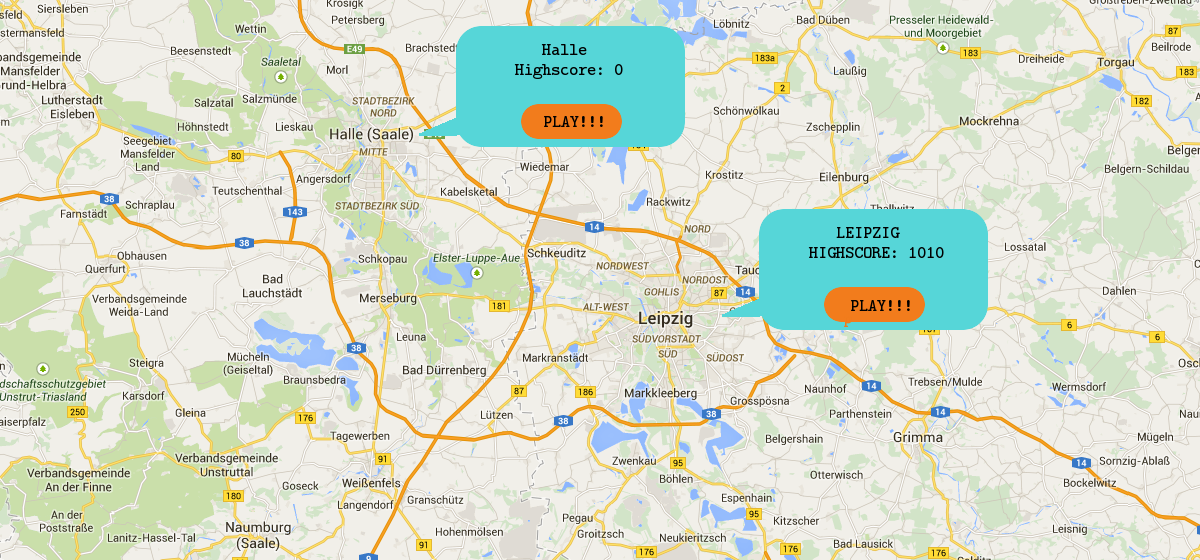
\includegraphics[scale=0.3]{gui.png}
%\caption{der rote Punkt bezeichnet unser gesuchtes Teilwort}
  \label{PNFs}
\end{figure} 
Das Interface soll erstmal einen Kartenausschnitt darstellen, an dem zu bestimmten Städten die Highscores angezeigt werden.
Drückt man auf den Play Button, statet das Spiel in dieser Stadt.

\begin{figure}[H]
  \centering
  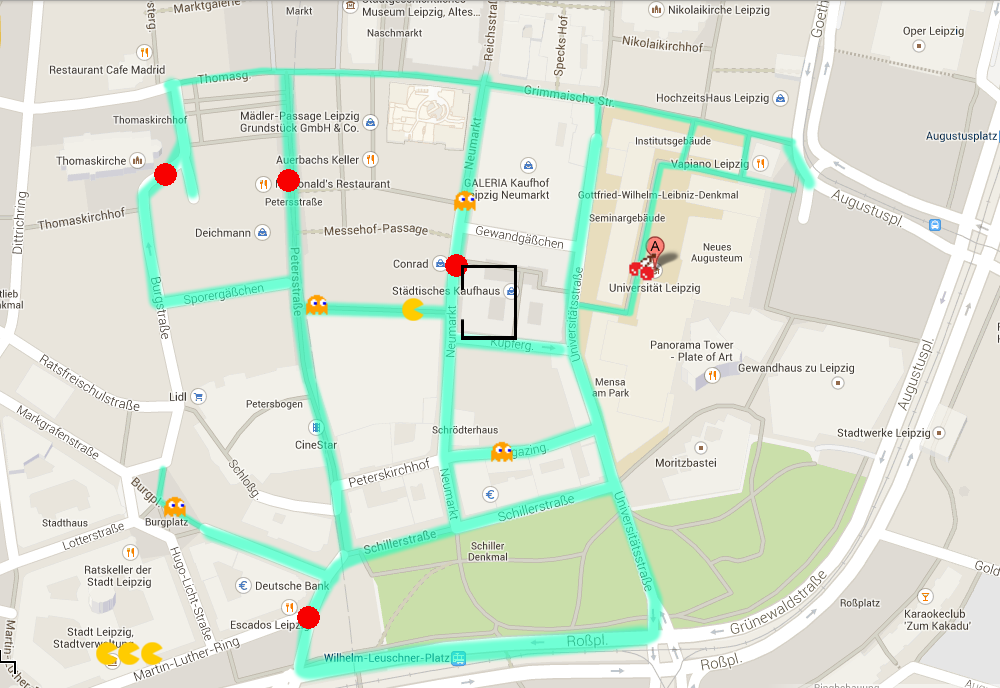
\includegraphics[scale=0.3]{pacman.png}
%\caption{der rote Punkt bezeichnet unser gesuchtes Teilwort}
  \label{PNFs}
\end{figure} 



\section{Webserver}
Der Webserver besteht aus der API und den Spiel-Daten die zum Spielen des Spiels an den Webclient übertragen werden.

\subsection{Database API als Datenbankzugriffsschicht}
Eine API (Schnittstelle zur Anwendungsprogrammierung) sorgt in unserem Fall dafür, dass die Daten aus der Datenbank an den Webclient übergeben werden. \\
Desweiteren sorgt die API dafür, dass Daten in die Datenbank übertragen werden oder falls gewünscht in der Datenbank geändert werden.  

\section{Datenserver}
\subsection{Datenbank}
Wir setzen einen Triplestore als Datenbank zum speichern von Spielkarten, Spielern und Highscores ein. \\
Alle Daten werden also als Tripel, bestehend aus Subjekt, Prädikat  
und Objekt gespeichert, wobei das Prädikat eine URI ist, um die Eindeutigkeit zu gewährleisten. Die Daten entsprechen dem RDF Standart. \\
Weitere Infos zu RDF, TipleStore bitte dem Recherchebericht entnehmen.

\section{relevante APIs}
\begin{itemize}
\item GoogleMaps API \\
	\url{https://developers.google.com/maps/} \\
	Diese API brauchen wir zur Darstellung der Karte.
\item LinkedGeoData API \\
	\url{http://linkedgeodata.org/OnlineAccess/SparqlEndpoints?v=n97} \\
	Diese API brachen für für semantische Daten und für die topologischen Daten der Karte.

\end{itemize}

\section{Vorprojekt}
\begin{itemize}
\item Webapplikation
\item Ausschnitt der Geo-Karte
\item auf einfachem Niveau mit der Karte zu agieren
\end{itemize}

Im Vorprojekt wird eine kleine Web Application erstellt, welche die Architektur minimal implementiert und es ermöglicht einen Punkt mit den Pfeiltasten über die Karte zu navigieren.

\section{Spieldetails}
\subsection{Minimalanforderungen}
%\end{frame}
%\begin{frame}{Minimalanforderungen Interface}
\begin{itemize}
\item Das Spiel findet auf einer realen Karte statt
\item Der Spieler kann den Kartenabschnitt auswählen
\item Der Spieler kann die verfügbaren Wege sehen /LF13/
\item Die Spielentitäten (Powerups, Coins Gespenster, Spielfigur) sollen angezeigt werden /LF14/
\item Wichtige Spielinformationen (Punkte, Leben) sollen angezeigt werden /LF15/
\end{itemize}
%\end{frame}
%\begin{frame}{Minimalanforderungen Gamedesign}
\begin{itemize}
\item Die Minimalanforderungen des Gamedesigns entsprechen der Spiellogik
\end{itemize}
%\end{frame}
%\begin{frame}{Minimalanforderungen Mapcreation}
\begin{itemize}
\item Dem Spieler steht eine Auswahl an vorgenerierten Karten zur Verfügung
\item Der Spieler kann die gleichen Level erneut spielen /LF41/
\item Semantische Daten haben Einfluss auf die Kartengenerierung /LF40/
\end{itemize}
\subsection{optionale Funktionalitäten}
%\end{frame}
%\begin{frame}{optionale Funktionalitäten Interface}
\begin{itemize}
\item Der Spieler kann einen beliebigen Ort auf der Welt auswählen
\item Der Spieler kann das Spielgeschehen hören
\item Der Spieler kann die Karten von anderen Spielern spielen
\end{itemize}
%\end{frame}
%\begin{frame}{optionale Funktionalitäten Gamedesign}
\begin{itemize}
\item Die optionalen Funktionalitäten des Gamedesigns entsprechen der optionalen Spiellogik
\end{itemize}
%\end{frame}
%\begin{frame}{optionale Funktionalitäten Highscore}
\begin{itemize}
\item Die Highscores der Spieler auf den Karten werden gespeichert und angezeigt
\item Der Spieler kann seinen Highscore auf sozialen Netzwerken veröffentlichen
\end{itemize}
%\end{frame}
%\begin{frame}{optionale Funktionalitäten Mapcreation}
\begin{itemize}
\item Eine Karte kann an einem beliebigen Ort erstellt werden
\end{itemize}
%\end{frame}
\subsection{Semantic Web}

\textbf{Wie wollen wir die Daten aus dem semantic Web in das Spiel einfließen lassen?}

\begin{itemize}
\item Wir wollen Anhand der Einwohnerzahl Städte selektieren.
\item Öffentliche Gebäude $\rightarrow$ an der Polizeistation spawnen die Geister, Powerups an Krankenhäusern
\item Tempolimit für die Geister?
\end{itemize}
\section{Qualitätssicherung}
\textbf{Unsere Qualitätsstandards:}
\begin{itemize}
\item Programmierstandards - Sun-Java-Codeconventions von 1997
\item Quelltextdokumentation
\item Testkonzepte - fehlerfreier Code durch	 JUnit, JSUnit
\end{itemize}
\par\bigskip	
\textbf{Eine
gute Dokumentation verkürzt die Einarbeitungszeit projektfremder
Entwickler in den Quellcode und erleichtert damit die Wartung und
Weiterentwicklung der Software.}

\section{Das angestrebte Ziel}
Die Minimalanforderungen sollen erfüllt sein und die Qualitätsstandards sollen eingehalten werden.

%\end{frame}
\end{document}